\documentclass[12pt,letterpaper, onecolumn]{exam}
\usepackage{amsmath}
\usepackage{amssymb}
\usepackage[lmargin=71pt, tmargin=1.2in]{geometry}
\usepackage{graphicx}%For centering solution box
\lhead{IND ENG 221\\}
\rhead{Kartikeya Sharma\\}
% \chead{\hline} % Un-comment to draw line below header
\thispagestyle{empty}   %For removing header/footer from page 1

\begin{document}

\begingroup  
    \centering
    \LARGE IND ENG 221\\
    \LARGE HW 4\\[0.5em]
    \large \today\\[0.5em]
    \large Kartikeya Sharma\par
    \large SID: 3037376860\par
\endgroup
\rule{\textwidth}{0.4pt}
\pointsdroppedatright   %Self-explanatory
\printanswers
\renewcommand{\solutiontitle}{\noindent\textbf{Ans:}\enspace}   %Replace "Ans:" with starting keyword in solution box



\section*{Q1}


A 1-month European put option on a non-dividend-paying stock is currently selling for \$2.50. The stock price is \$47, the strike price is \$50, and the risk-free interest rate is 6\% per annum. What opportunities are there for an arbitrageur?
\subsection*{Step 1: No-Arbitrage Lower Bound for the Put Option}

The no-arbitrage lower bound for a European put option is:

\[
P \geq \max \left( 0, K e^{-rT} - S \right)
\]

Given:
- Strike price \( K = 50 \, \text{USD} \)
- Stock price \( S = 47 \, \text{USD} \)
- Risk-free interest rate \( r = 0.06 \)
- Time to maturity \( T = \frac{1}{12} \, \text{years} \)

We first calculate the present value of the strike price:

\[
K e^{-rT} = 50 e^{-0.06 \times \frac{1}{12}} = 50 \times e^{-0.005} = 50 \times 0.995 = 49.75 \, \text{USD}
\]

Now, we calculate the no-arbitrage lower bound for the put option:

\[
P \geq \max(0, 49.75 - 47) = \max(0, 2.75) = 2.75 \, \text{USD}
\]

\subsection*{Step 2: Comparison with the Market Price}

The market price of the put option is \$2.50, which is below the no-arbitrage lower bound of \$2.75. This indicates that the put option is underpriced and provides an arbitrage opportunity.

\subsection*{Step 3: Arbitrage Strategy}

The arbitrageur can take the following actions:

1. Buy the underpriced put option for \$2.50.
2. Short the stock at the current price of \$47.
3. Lend the present value of the strike price (\$49.75) at the risk-free rate.

\subsection*{Step 4: Arbitrage Payoff at Expiration}

There are two possible scenarios at expiration:

- If the stock price is below the strike price (\$50), the arbitrageur exercises the put option and buys the stock at \$50 to cover the short position. The arbitrageur profits from the difference between \$49.75 and \$47, minus the cost of the put.
- If the stock price is above \$50, the put expires worthless, and the arbitrageur profits from the short sale and the interest earned on the loan.

\section*{Conclusion}

The put option is underpriced, and the arbitrageur can profit by buying the put, shorting the stock, and lending the present value of the strike price at the risk-free rate.


    \newpage
    
\section*{Q2}

The price of a European call that expires in 6 months and has a strike price of \$30 is \$2. The underlying stock price is \$29, and a dividend of \$0.50 is expected in 2 months and again in 5 months. Risk-free interest rates (all maturities) are 10\%. What is the price of a European put option that expires in 6 months and has a strike price of \$30?

\section*{Solution}

\subsection*{Step 1: Put-Call Parity Formula}

The put-call parity relationship for European options with dividends is given by:

\[
C + K e^{-rT} = P + (S - PV_{\text{dividends}})
\]

Where:
- \( C = 2 \, \text{USD} \) is the call price.
- \( K = 30 \, \text{USD} \) is the strike price.
- \( S = 29 \, \text{USD} \) is the stock price.
- \( r = 0.10 \) is the risk-free interest rate.
- \( T = 6/12 = 0.5 \, \text{years} \).
- \( PV_{\text{dividends}} \) is the present value of the dividends.

\subsection*{Step 2: Present Value of the Dividends}

The dividends are expected in 2 months and 5 months. The present value of the first dividend is:

\[
PV_{\text{dividend1}} = 0.50 e^{-0.10 \times \frac{1}{6}} = 0.50 e^{-0.01667} = 0.50 \times 0.9835 = 0.4917 \, \text{USD}
\]

The present value of the second dividend is:

\[
PV_{\text{dividend2}} = 0.50 e^{-0.10 \times \frac{5}{12}} = 0.50 e^{-0.04167} = 0.50 \times 0.9592 = 0.4796 \, \text{USD}
\]

Thus, the total present value of the dividends is:

\[
PV_{\text{dividends}} = 0.4917 + 0.4796 = 0.9713 \, \text{USD}
\]

\subsection*{Step 3: Present Value of the Strike Price}

The present value of the strike price is:

\[
K e^{-rT} = 30 e^{-0.10 \times 0.5} = 30 \times e^{-0.05} = 30 \times 0.9512 = 28.536 \, \text{USD}
\]

\subsection*{Step 4: Calculate the Put Price}

Using the put-call parity formula:

\[
P = C + K e^{-rT} - (S - PV_{\text{dividends}})
\]

Substituting the values:

\[
P = 2 + 28.536 - (29 - 0.9713) = 2 + 28.536 - 28.0287 = 2.5073 \, \text{USD}
\]

Thus, the price of the European put option is approximately \$2.51.

\newpage

    \pagebreak %Not necessary
    
\section*{Q3}

Suppose that \( c_1 \), \( c_2 \), and \( c_3 \) are the prices of European call options with strike prices \( K_1 \), \( K_2 \), and \( K_3 \), respectively, where \( K_3 > K_2 > K_1 \) and \( K_3 - K_2 = K_2 - K_1 \). All options have the same maturity. Show that:

\[
c_2 \leq \frac{c_1 + c_3}{2}
\]

\section*{Solution}

\subsection*{Step 1: Consider a Portfolio}

We consider a portfolio consisting of:
- Long one call option with strike price \( K_1 \) (price \( c_1 \)),
- Long one call option with strike price \( K_3 \) (price \( c_3 \)),
- Short two call options with strike price \( K_2 \) (price \( c_2 \)).

\subsection*{Step 2: Payoff at Maturity}

Let \( S_T \) denote the stock price at maturity. The payoff of the portfolio depends on \( S_T \), and we consider different cases:

\textbf{Case 1: \( S_T \leq K_1 \)}

All options expire worthless, and the portfolio payoff is:

\[
\text{Payoff} = 0
\]

\textbf{Case 2: \( K_1 < S_T \leq K_2 \)}

The option with strike price \( K_1 \) is in the money, and its payoff is \( S_T - K_1 \). The options with strike prices \( K_2 \) and \( K_3 \) are out of the money, so their payoffs are 0. The portfolio payoff is:

\[
\text{Payoff} = S_T - K_1
\]

\textbf{Case 3: \( K_2 < S_T \leq K_3 \)}

The options with strike prices \( K_1 \) and \( K_2 \) are in the money, and their payoffs are \( S_T - K_1 \) and \( S_T - K_2 \), respectively. The option with strike price \( K_3 \) is out of the money. The portfolio payoff is:

\[
\text{Payoff} = (S_T - K_1) + (S_T - K_3) - 2(S_T - K_2) = 0
\]

\textbf{Case 4: \( S_T > K_3 \)}

All options are in the money. The portfolio payoff is:

\[
\text{Payoff} = (S_T - K_1) + (S_T - K_3) - 2(S_T - K_2) = 0
\]

\subsection*{Step 3: Portfolio Payoff is Non-Negative}

The portfolio payoff is always non-negative. By the no-arbitrage condition, the value of the portfolio today must also be non-negative. The portfolio value today is:

\[
c_1 + c_3 - 2c_2
\]

Thus, we have:

\[
c_1 + c_3 - 2c_2 \geq 0
\]

Rearranging this inequality gives:

\[
c_2 \leq \frac{c_1 + c_3}{2}
\]

\subsection*{Conclusion}

We have shown that:

\[
c_2 \leq \frac{c_1 + c_3}{2}
\]


    \newpage


    
\section*{Q4}

A trader creates a bear spread by selling a 6-month put option with a \$25 strike price for \$2.15 and buying a 6-month put option with a \$29 strike price for \$4.75. What is the initial investment? What is the total payoff (excluding the initial investment) when the stock price in 6 months is (a) \$23, (b) \$28, and (c) \$33?

\section*{Solution}

\subsection*{Step 1: Initial Investment}

The initial investment is the net cost of the strategy:

\[
\text{Initial Investment} = \text{Cost of Buying Put} - \text{Premium from Selling Put}
\]
\[
\text{Initial Investment} = 4.75 - 2.15 = 2.60 \, \text{USD}
\]

Thus, the initial investment is \$2.60.

\subsection*{Step 2: Payoff Calculation}

We calculate the payoff for different stock prices at expiration.

\textbf{Case (a): Stock price = \$23}

\begin{itemize}
    \item Payoff from buying the \$29 put: \( 29 - 23 = 6 \, \text{USD} \)
    \item Payoff from selling the \$25 put: \( 25 - 23 = 2 \, \text{USD} \)
\end{itemize}

Total payoff:
\[
\text{Total Payoff} = 6 - 2 = 4 \, \text{USD}
\]

\textbf{Case (b): Stock price = \$28}

\begin{itemize}
    \item Payoff from buying the \$29 put: \( 29 - 28 = 1 \, \text{USD} \)
    \item Payoff from selling the \$25 put: \( 0 \, \text{USD} \)
\end{itemize}

Total payoff:
\[
\text{Total Payoff} = 1 - 0 = 1 \, \text{USD}
\]

\textbf{Case (c): Stock price = \$33}

\begin{itemize}
    \item Payoff from buying the \$29 put: \( 0 \, \text{USD} \)
    \item Payoff from selling the \$25 put: \( 0 \, \text{USD} \)
\end{itemize}

Total payoff:
\[
\text{Total Payoff} = 0 - 0 = 0 \, \text{USD}
\]

\subsection*{Summary of Payoffs}

- Initial investment: \$2.60
- Total payoff when stock price is \$23: \$4
- Total payoff when stock price is \$28: \$1
- Total payoff when stock price is \$33: \$0

\newpage

\section*{Q5}

A diagonal spread is created by buying a call with strike price \( K_2 \) and exercise date \( T_2 \), and selling a call with strike price \( K_1 \) and exercise date \( T_1 \), where \( T_2 > T_1 \). Draw a diagram showing the profit from the spread at time \( T_1 \) when:
\begin{itemize}
    \item (a) \( K_2 > K_1 \)
    \item (b) \( K_2 < K_1 \)
\end{itemize}

\section*{Solution}

Step 1: Strategy Payoff Explanation

The diagonal spread consists of:
\begin{itemize}
    \item Buying a call with strike price \( K_2 \) and later expiration \( T_2 \),
    \item Selling a call with strike price \( K_1 \) and earlier expiration \( T_1 \).
\end{itemize}

We analyze the payoffs at time \( T_1 \), which is when the short call expires.

Case (a): \( K_2 > K_1 \)

- If the stock price \( S_{T_1} \leq K_1 \): Both options are out of the money, so the profit is zero.
- If \( K_1 < S_{T_1} < K_2 \): The short call is in the money, so there is a loss of \( S_{T_1} - K_1 \). The long call remains out of the money.
- If \( S_{T_1} \geq K_2 \): Both calls are in the money, but the long call's profit offsets the short call's loss, capping the total loss.

Case (b): \( K_2 < K_1 \)

- If the stock price \( S_{T_1} \leq K_2 \): Both options are out of the money, so the profit is zero.
- If \( K_2 < S_{T_1} < K_1 \): The long call is in the money, giving a profit of \( S_{T_1} - K_2 \), while the short call remains out of the money.
- If \( S_{T_1} \geq K_1 \): Both calls are in the money, limiting the profit as the short call's loss offsets the long call's gain.

Step 2: Profit Diagrams

The following image shows the profit diagrams for both cases:

\begin{figure}[h!]
    \centering
    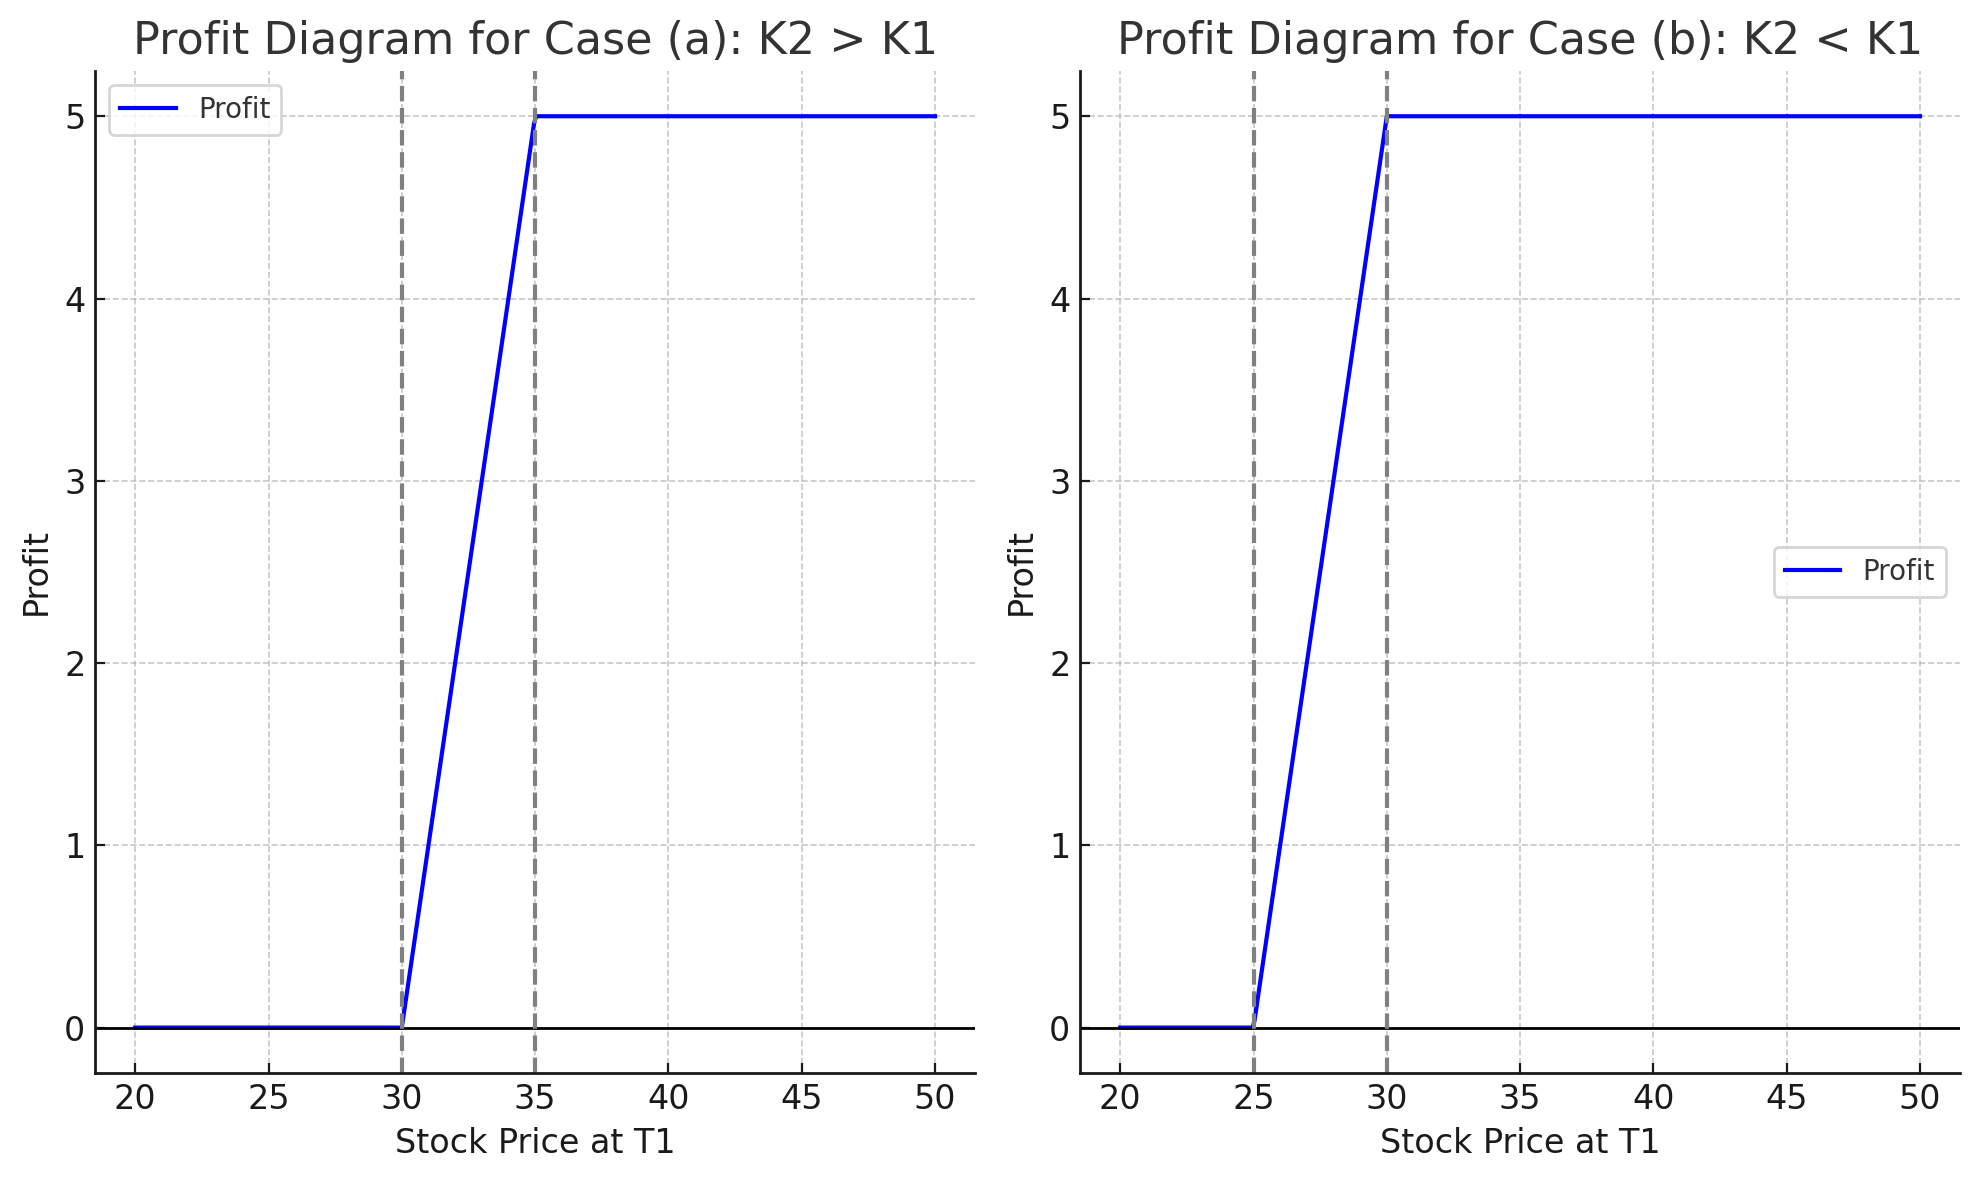
\includegraphics[width=0.8\textwidth]{output.png}
    \caption{Profit Diagram for Diagonal Spread}
\end{figure}

\section*{Conclusion}

The diagrams illustrate the profit structure for the diagonal spread at time \( T_1 \) for:

\begin{itemize}
    \item Case (a): \( K_2 > K_1 \): The maximum loss is capped after \( S_{T_1} \) exceeds \( K_2 \).
    \item Case (b): \( K_2 < K_1 \): The profit is maximized between \( K_2 \) and \( K_1 \), then capped.
\end{itemize

\end{document}